\documentclass{article}
\usepackage{iclr2027_conference,times}
\usepackage{amsmath,amssymb,amsthm,booktabs,graphicx,microtype}
\usepackage{hyperref,url}
\usepackage{array}
%% Generated by python -m src.report; do not edit empirical numbers.
\newcommand{\HelmN}{79}
\newcommand{\HelmD}{57}
\newcommand{\OllN}{4496}
\newcommand{\OllD}{6}
\newcommand{\OllRawN}{4576}
\newcommand{\OllDuplicates}{79}
\newcommand{\OllFlagged}{1}
\newcommand{\HelmCommon}{77}
\newcommand{\HelmUnitMeanK}{17.12}
\newcommand{\HelmUnitMeanMass}{14.56}
\newcommand{\HelmUnitMedianK}{19.82}
\newcommand{\HelmUnitMedianMass}{3.44}
\newcommand{\HelmUnitGeometricK}{17.35}
\newcommand{\HelmUnitGeometricMass}{14.10}
\newcommand{\HelmUnitMinimumK}{13.52}
\newcommand{\HelmUnitMinimumMass}{3.09}
\newcommand{\HelmUnitMedLess}{14.3}
\newcommand{\HelmUnitMedMore}{83.1}
\newcommand{\HelmUnitMassLess}{100.00}
\newcommand{\HelmUnitOneMean}{2.6}
\newcommand{\HelmUnitOneMedian}{2.6}
\newcommand{\HelmObservedMeanK}{34.96}
\newcommand{\HelmObservedMeanMass}{14.56}
\newcommand{\HelmObservedMedianK}{19.82}
\newcommand{\HelmObservedMedianMass}{3.72}
\newcommand{\HelmObservedGeometricK}{34.13}
\newcommand{\HelmObservedGeometricMass}{14.29}
\newcommand{\HelmObservedMinimumK}{13.52}
\newcommand{\HelmObservedMinimumMass}{3.09}
\newcommand{\HelmObservedMedLess}{97.4}
\newcommand{\HelmObservedMedMore}{0.0}
\newcommand{\HelmObservedMassLess}{100.00}
\newcommand{\HelmObservedOneMean}{0.0}
\newcommand{\HelmObservedOneMedian}{2.6}
\newcommand{\OllCommon}{4493}
\newcommand{\OllUnitMeanK}{2.36}
\newcommand{\OllUnitMeanMass}{30.25}
\newcommand{\OllUnitMedianK}{2.85}
\newcommand{\OllUnitMedianMass}{18.44}
\newcommand{\OllUnitGeometricK}{2.98}
\newcommand{\OllUnitGeometricMass}{25.79}
\newcommand{\OllUnitMinimumK}{3.66}
\newcommand{\OllUnitMinimumMass}{8.52}
\newcommand{\OllUnitMedLess}{0.0}
\newcommand{\OllUnitMedMore}{47.4}
\newcommand{\OllUnitMassLess}{99.93}
\newcommand{\OllUnitOneMean}{9.1}
\newcommand{\OllUnitOneMedian}{0.8}
\newcommand{\OllObservedMeanK}{3.88}
\newcommand{\OllObservedMeanMass}{30.25}
\newcommand{\OllObservedMedianK}{3.24}
\newcommand{\OllObservedMedianMass}{18.81}
\newcommand{\OllObservedGeometricK}{4.65}
\newcommand{\OllObservedGeometricMass}{26.99}
\newcommand{\OllObservedMinimumK}{3.66}
\newcommand{\OllObservedMinimumMass}{8.52}
\newcommand{\OllObservedMedLess}{62.5}
\newcommand{\OllObservedMedMore}{0.2}
\newcommand{\OllObservedMassLess}{99.93}
\newcommand{\OllObservedOneMean}{0.2}
\newcommand{\OllObservedOneMedian}{0.8}
\newcommand{\OllRawObservedMedLess}{11.0}
\newcommand{\HelmObservedMedianWeakK}{43.31}
\newcommand{\MixedSwitchers}{64}
\newcommand{\MixedQOne}{0.492}
\newcommand{\MixedMedian}{0.563}
\newcommand{\MixedQThree}{0.644}
\newcommand{\HelmUnitQuarterMeanFeasible}{9.1}
\newcommand{\HelmUnitQuarterMedianFeasible}{11.7}
\newcommand{\HelmUnitHalfMeanFeasible}{49.4}
\newcommand{\HelmUnitHalfMedianFeasible}{50.6}
\newcommand{\HelmUnitThreeQuarterMeanFeasible}{97.4}
\newcommand{\HelmUnitThreeQuarterMedianFeasible}{93.5}
\newcommand{\HelmObservedQuarterMeanFeasible}{2.6}
\newcommand{\HelmObservedQuarterMedianFeasible}{3.9}
\newcommand{\HelmObservedHalfMeanFeasible}{2.6}
\newcommand{\HelmObservedHalfMedianFeasible}{6.5}
\newcommand{\HelmObservedThreeQuarterMeanFeasible}{18.2}
\newcommand{\HelmObservedThreeQuarterMedianFeasible}{16.9}
\newcommand{\OllUnitQuarterMeanFeasible}{12.2}
\newcommand{\OllUnitQuarterMedianFeasible}{9.3}
\newcommand{\OllUnitHalfMeanFeasible}{96.8}
\newcommand{\OllUnitHalfMedianFeasible}{75.0}
\newcommand{\OllUnitThreeQuarterMeanFeasible}{100.0}
\newcommand{\OllUnitThreeQuarterMedianFeasible}{100.0}
\newcommand{\OllObservedQuarterMeanFeasible}{0.1}
\newcommand{\OllObservedQuarterMedianFeasible}{0.9}
\newcommand{\OllObservedHalfMeanFeasible}{3.5}
\newcommand{\OllObservedHalfMedianFeasible}{10.1}
\newcommand{\OllObservedThreeQuarterMeanFeasible}{58.1}
\newcommand{\OllObservedThreeQuarterMedianFeasible}{75.3}
\newcommand{\RunWallSeconds}{112.7}
\newcommand{\RunCpuSeconds}{111.9}
\newcommand{\RunPeakMiB}{378.4}
\newcommand{\WitnessCases}{109800}
\newcommand{\RawFiles}{61}
\newcommand{\RawMB}{8.97}

\newtheorem{proposition}{Proposition}
\newtheorem{lemma}{Lemma}
\newcommand{\R}{\mathbb{R}}
\newcommand{\ind}{\mathbf{1}}
\newcommand{\K}{K^*}
\newcommand{\C}{C^*}
\newcommand{\eps}{\varepsilon}
\newcommand{\mean}{\mathrm{mean}}
\newcommand{\med}{\mathrm{med}}
\title{Which Tasks Must Change to Win?\\Exact Score-Space Audits of Multi-Task Aggregation}
\author{Autonomous research report\\Prepared for a user-specified research task}
\iclrfinalcopy
% Preserve the official layout while avoiding a false publication/submission claim.
\lhead{Independent research report in ICLR 2027 format; not submitted}
\begin{document}
\maketitle
\begin{abstract}
How much targeted improvement would make a model first on a multi-task leaderboard?
We study this question as a conditional optimization problem on public score matrices,
without estimating training responses. Investment is measured either by the number
of improved tasks or by total score increase. We give exact algorithms for arithmetic
mean, median, geometric mean, and minimum aggregation, including bounded and
infeasible improvements. On \HelmN{} models across \HelmD{} HELM--MMLU subjects
and \OllN{} Open LLM models across \OllD{} evaluations, the apparent ordering of
mean and median reverses with the improvement ceiling. With perfect scores allowed,
median requires more changed tasks than mean for \HelmUnitMedMore\% and
\OllUnitMedMore\% of common challengers, respectively. With ceilings set to each
task's best observed score, median requires fewer tasks for \HelmObservedMedLess\%
and \OllObservedMedLess\%. Yet median requires less total score increase for nearly
every challenger. Task resampling and alternative score normalization further qualify
these comparisons. Thus no aggregation rule has a universal investment advantage:
the ceiling, cost definition, and task composition are part of the answer.
These are reproducible score-space certificates, not estimates of data or compute
needed to train a winning model.
\end{abstract}

\section{Introduction}
\label{sec:intro}
A multi-task leaderboard turns a vector of task scores into one rank. This creates
two distinct questions: what abilities should count, and how easily could a developer
change the winning rank by concentrating improvement on selected tasks? The latter
matters when benchmark-aligned data curation or post-training improves measured
performance without comparable improvements elsewhere. Experiments on benchmark
leakage and rephrased test samples establish that this concern is substantive
\citep{zhou2023cheater,yang2023rephrased}. They do not identify the response of every
model on every task, however. A score table alone cannot tell us how many training
examples, tokens, or GPU hours would buy a given improvement.

We therefore ask a narrower, identifiable question. Conditional on a specified set
of task-wise attainable scores, what is the least score-space intervention that makes
a fixed model first while its rivals stay fixed? We measure intervention in two ways:
the number of affected tasks and the average absolute increase across tasks. Both
are useful audit quantities, but neither is a measured training cost. The first
captures task-level setup or data-acquisition overhead; the second captures the
amount of score movement. Their disagreement is itself a result.

One might expect a median to resist targeting because it ignores extreme scores.
That intuition omits both the target's starting vector and the incumbent's threshold.
An already strong model may need to move only one score across a median boundary.
Conversely, a target with many scores just below that boundary may need numerous
small changes, while a mean can be shifted through one large change. The familiar
question of how many arbitrary observations destroy a location estimate is different
from making one particular bounded vector beat the best competing vector.

Our main empirical finding is a reversal that holds on the same matrices and the
same target cohorts. Allowing selected scores to reach one gives median a larger
average task count than mean on both panels. Restricting ceilings to the best scores
already observed in each task reverses that comparison for most targets. The second
ceiling is a sensitivity scenario, not an assertion that borrowing another model's
best score is achievable. Both scenarios are deliberately explicit; treating either
as ground truth about training would be unwarranted.

The contributions are threefold. First, we formulate minimum investment with fixed
rivals, bounded improvements, ties, and unreachable winners. Second, we provide
exact, transparent solvers and characterize when the same subset is optimal across
symmetric aggregation rules. A constructive example shows how changing only the
ceiling reverses the ordering. Third, we audit two public snapshots with shared
challenger cohorts, alternative investment units, weaker responses, score-scale and
row-selection controls, and task-composition perturbations. Our claims concern
these audited settings and inspected literature; they do not assert exhaustive priority.

\section{Related work}
\label{sec:related}
MMLU evaluates knowledge over many subjects \citep{hendrycks2021mmlu}; HELM emphasizes
standardized and transparent evaluation across scenarios and metrics
\citep{liang2023helm}. We use HELM's later MMLU score release and the public Open LLM
Leaderboard table \citep{helm2025data,oll2025contents}. Our macro aggregation over
HELM subjects is an explicit counterfactual scoring rule, not an attempt to reproduce
every displayed HELM summary. The benchmark lottery shows that task choice changes
relative algorithm performance \citep{dehghani2021lottery}; here task resampling tests
whether an investment comparison survives a change of composition.

\citet{lanctot2023social} treat tasks as voters and study ordinal evaluation rules,
including consistency properties and cycles. We examine four cardinal aggregators
whose rivals' aggregate scores remain fixed when the target changes. Thus our
threshold reduction does not directly cover Borda, pairwise tournaments, or other
rules under which changing one model also changes competitors' scores. Election
bribery asks whether bounded intervention can make a preferred candidate win
\citep{faliszewski2006bribery}. Our intervention changes only the target's cardinal
coordinates, with a box constraint rather than arbitrary ballot changes.

\citet{chen2026incentives} model a benchmark designer and multiple developers in a
Stackelberg game and analyze equilibrium incentives under strategic post-training.
We instead solve a unilateral, static, finite-table optimization problem; no
equilibrium, latent ability, or post-training response is inferred.
Contamination experiments \citep{zhou2023cheater,yang2023rephrased} motivate targeted
improvement but also caution against treating independent, harmless score gains as
an empirical law. These differences delimit our contribution rather than establish
that the broader strategic phenomenon is new.

\section{Problem and assumptions}
\label{sec:setup}
Let $X\in[0,1]^{n\times d}$ contain complete, higher-is-better scores. For target
$i$, write $x=X_i$ and let $g$ be the aggregation rule. The competing threshold is
\begin{equation}
 t_{i,g}=\max_{\ell\ne i}g(X_\ell)+\eps .
 \label{eq:threshold}
\end{equation}
Our primary convention is co-first place, $\eps=0$. A sensitivity analysis uses
$\eps=10^{-6}$ on the unit score scale, a finite positive winning margin rather
than an unattained strict-inequality infimum. Numerical comparisons use a
$10^{-12}$ tolerance.

\paragraph{Feasible improvement.}
The target may choose any $y$ with $x\le y\le u$. We parameterize
\begin{equation}
 u_j=x_j+\rho(c_j-x_j),\qquad
 c_j=1\ \text{(unit ceiling)},\quad\text{or}\quad
 c_j=\max_\ell X_{\ell j}\ \text{(observed ceiling)},
 \label{eq:cap}
\end{equation}
where $\rho\in\{0.1,0.25,0.5,0.75,1\}$ specifies the fraction of available headroom.
The unit ceiling supplies a deliberately optimistic limit. The observed ceiling
keeps gains within the snapshot's empirical per-task envelope, but a vector combining
different models' task maxima need not correspond to any trainable model. We do not
fit $\rho$ to data or interpret it as a learning rate.

\paragraph{Investment.}
We compute two separate optima:
\begin{align}
 \K_g(x,u,t)&=\min_{x\le y\le u}\{\|y-x\|_0:g(y)\ge t\},\label{eq:k}\\
 \C_g(x,u,t)&=\min_{x\le y\le u}\{d^{-1}\|y-x\|_1:g(y)\ge t\}.\label{eq:c}
\end{align}
An infeasible optimum is $+\infty$. $K^*$ counts selected tasks, regardless of the
size of their gains. $C^*$ allows partial increases and is reported in average
percentage points. The two optimizers may differ. Task costs are uniform: neither
metric equates a 57-subject MMLU task with a whole Open LLM evaluation in training
effort. Fractions $K^*/d$ allow descriptive plots, not a conversion between those units.

\paragraph{Scope of the model.}
The developer knows all snapshot scores and the rule, rivals do not respond, gains
on selected tasks can be controlled independently, and other scores do not change.
These assumptions isolate the aggregation effect. They exclude transfer, forgetting,
coupled learning curves, hidden tests, noisy score estimation, and multi-developer
competition. Under these assumptions the unit-ceiling $K^*$ is an optimistic lower
bound for any smaller attainable box. It is not such a bound on the number of
training domains if training on one domain also improves several other coordinates.

\paragraph{Aggregation rules.}
We study the arithmetic mean $d^{-1}\sum_jy_j$, the conventional median (averaging
the middle pair when $d$ is even), the geometric mean $(\prod_jy_j)^{1/d}$ with
zero preserved, and the minimum $\min_jy_j$. The latter two emphasize weak tasks in
different ways. All are symmetric and coordinatewise nondecreasing. We give no
normative ranking of them: a minimum and a mean encode different notions of merit.
Each rule uses its own best rival in Equation~\ref{eq:threshold}.

\section{Exact investment certificates}
\label{sec:methods}
The optimization is small enough to solve exactly for the two audited dimensions.
The following results also explain why its answer depends on the intervention model.
Proofs and continuous-cost algorithms are in Appendix~\ref{app:proofs}.

\begin{proposition}[Endpoint reduction and a shared-ceiling optimum]
\label{prop:endpoint}
For any coordinatewise nondecreasing $g$, a minimum-support feasible intervention
can be taken to have $y_j\in\{x_j,u_j\}$. If $u_j=c\ge\max_jx_j$ for every $j$ and
$g$ is also symmetric, raising the $k$ smallest original scores to $c$ maximizes
$g(y)$ among all interventions on at most $k$ coordinates.
\end{proposition}
The second statement follows because replacing a larger original score instead of
a smaller one leaves a smaller unchanged coordinate; exchanging the choice weakly
increases every sorted coordinate. Consequently, at the full unit ceiling,
``lowest score first'' is an optimal strategy for all four rules. Their different
budgets then reflect different winning boundaries, not different task-selection
heuristics. With partial response or heterogeneous ceilings this conclusion need
not hold.

\begin{proposition}[Exact support costs]
\label{prop:support}
Let $\Delta=dt-\sum_jx_j$ and let $a_{(1)}\ge\cdots\ge a_{(d)}$ sort the gains
$a_j=u_j-x_j$. For the mean,
\begin{equation}
 \K_\mean=\min\{k:\textstyle\sum_{r=1}^k a_{(r)}\ge\Delta\}.
 \label{eq:mean}
\end{equation}
The geometric mean has the same prefix form in log scores, after mandatory changes
to every zero coordinate when $t>0$. For an odd number $d=2m-1$ of tasks, define
$A=\#\{j:x_j\ge t\}$ and $B=\#\{j:u_j\ge t\}$. Then
\begin{equation}
 \K_\med=\begin{cases}(m-A)_+,&B\ge m,\\+\infty,&B<m.\end{cases}
 \label{eq:median}
\end{equation}
For the minimum, every coordinate below $t$ must be changed, and any $u_j<t$
makes winning infeasible. For any rule, feasibility with unrestricted support is
equivalent to $g(u)\ge t$.
\end{proposition}
Mean and log-mean costs require sorting, $O(d\log d)$; odd median and minimum
require counting, $O(d)$. On the six-task panel, all $2^6$ endpoint subsets are
enumerated for the even median. This avoids substituting a nonstandard lower or
upper median for the official mathematical convention. The best feasible subset
is retained as a witness.

Equation~\ref{eq:median} also identifies a useful invariance: as long as at least
$m$ caps cross the median threshold, their exact magnitudes do not change $K^*_\med$.
The mean instead responds to the entire distribution of gains $u_j-x_j$. Reducing
headroom can therefore change the mean's budget without changing the median's.
In particular, at full response with co-first allowed, observed ceilings always
permit the best rival's score vector. Thus odd-median and minimum support costs
must equal their unit-ceiling costs; the even median has no such guarantee.
No claim of a universal ordering is possible.

\begin{proposition}[A ceiling-only reversal]
\label{prop:flip}
There exists a single leaderboard, a fixed challenger, and fixed competing models
such that $\K_\mean<\K_\med$ under the unit ceiling but
$\K_\mean>\K_\med$ under the observed ceiling. This holds both for co-first place
and for a sufficiently small positive winning margin.
\end{proposition}
For a concrete proof construction, take target $(.59,.59,.59)$, incumbent
$(.60,.60,.60)$, and three specialist rivals whose only nonzero coordinate is
$.604$, one on each task. Both thresholds are $.60$. Unit ceilings give budgets
$(K^*_\mean,K^*_\med)=(1,2)$; observed ceilings give $(3,2)$. These are algebraic
counterexamples, not empirical benchmark observations. Appendix~\ref{app:proofs}
also gives an example with median cheaper than mean at the unit ceiling.

For continuous investment, the mean has $C^*_\mean=(t-g_\mean(x))_+$ whenever
feasible. The odd median sums the $m$ smallest feasible deficits $(t-x_j)_+$,
including zero deficits, then divides by $d$. The minimum sums all deficits.
The geometric solution raises low coordinates to a common level, subject to
their caps, as derived from the log constraint. An exact small-dimensional
algorithm for the even median is given in Appendix~\ref{app:mass}.
There is no reason for the ordering in task count to match that in score mass.

\section{Empirical audit}
\label{sec:experiments}
\subsection{Data, targets, and validation}
\label{sec:data}
\textbf{HELM--MMLU.} We use release v1.13.0, dated January 10, 2025, downloaded
November 2, 2026. Its subject JSON summaries yield \HelmN{} evaluated model entries
with all \HelmD{} subject exact-match scores. Model/protocol identifiers are taken
from run-spec metadata, not display labels. No entry is dropped for missing scores.
Subjects receive equal weight in the primary audit; evaluation-instance weighting
is a separate control (Appendix~\ref{app:controls}).

\textbf{Open LLM.} We use the March 20, 2025 contents snapshot pinned to commit
\texttt{9c09a7c}\ldots\texttt{afa2}. The downloaded table has \OllRawN{} rows over
IFEval, BBH, MATH level 5, GPQA, MuSR, and MMLU-Pro. We remove \OllFlagged{} flagged
entry, then choose one record per model name by a score-independent precision
priority and lexicographic evaluation identifier, removing \OllDuplicates{} extra
records. The resulting \OllN{} models are complete on all six tasks. We divide
displayed normalized scores by 100; their equal-weight mean exactly reproduces
the provided average. Raw metric columns and all unflagged evaluation entries are
separate sensitivity panels. We do not assume that heterogeneous metrics have a
shared scientific utility merely because they share a numeric range.

For paired rule comparisons we fix a \emph{common challenger cohort}: entries
that are not initially co-first under any of the four rules. This leaves
\HelmCommon{} HELM and \OllCommon{} Open LLM targets. Rival sets still contain all
retained entries, including initial winners. Thus no rule gains an easier target
sample by excluding its own losers. The same cohort is used across ceilings,
response strengths, and winning margins. A top-20\% cohort uses original mean
rank, with the same cross-rule exclusion. All snapshots, checksums, row-selection
rules, and model-level results accompany the artifact.

All calculations are deterministic except explicitly seeded perturbations and
random-order baselines. Small matrices are checked against exhaustive subset
search; median mass is checked against independently formulated linear programs
over score orderings, and geometric mass against constrained numerical
optimization. Across \WitnessCases{} primary-panel cases we audit endpoint
witnesses when feasible. Optimality on the full panels follows from the formulas
or full enumeration, rather than a heuristic solver. The main run used
\RunCpuSeconds{} CPU seconds and \RunPeakMiB{} MiB peak resident memory.

\subsection{The ceiling reverses the task-count comparison}
\label{sec:primary}
Table~\ref{tab:support} reports finite-census averages of exact minimum task counts;
all targets are feasible at $\rho=1$. Under unit ceilings, mean needs fewer tasks
than median for \HelmUnitMedMore\% of HELM challengers and \OllUnitMedMore\% of
Open LLM challengers. Median is cheaper for \HelmUnitMedLess\% and
\OllUnitMedLess\%, respectively. Under observed ceilings, median becomes cheaper
for \HelmObservedMedLess\% and \OllObservedMedLess\%. These are paired comparisons
for the same models, not comparisons of independently averaged rank groups.

\begin{table}[t]
\centering\small\setlength{\tabcolsep}{3pt}
\begin{tabular}{llrrrrrr}
\toprule
Panel & Ceiling & Mean & Median & Geom. & Min. & $K_{\rm med}<K_{\rm mean}$ (\%) & $>$ (\%) \\
\midrule
HELM--MMLU & Unit & 17.12 & 19.82 & 17.35 & 13.52 & 14.3 & 83.1 \\
HELM--MMLU & Observed & 34.96 & 19.82 & 34.13 & 13.52 & 97.4 & 0.0 \\
Open LLM & Unit & 2.36 & 2.85 & 2.98 & 3.66 & 0.0 & 47.4 \\
Open LLM & Observed & 3.88 & 3.24 & 4.65 & 3.66 & 62.5 & 0.2 \\
\bottomrule
\end{tabular}

\caption{Mean minimum task count $K^*$ at $\rho=1$, co-first convention.
The final columns report the fraction of common challengers for which median
costs fewer or more tasks than mean. Equal cases make up the remainder. Each
panel uses its own task unit; counts should not be compared as training costs.}
\label{tab:support}
\end{table}

\begin{figure}[t]
\centering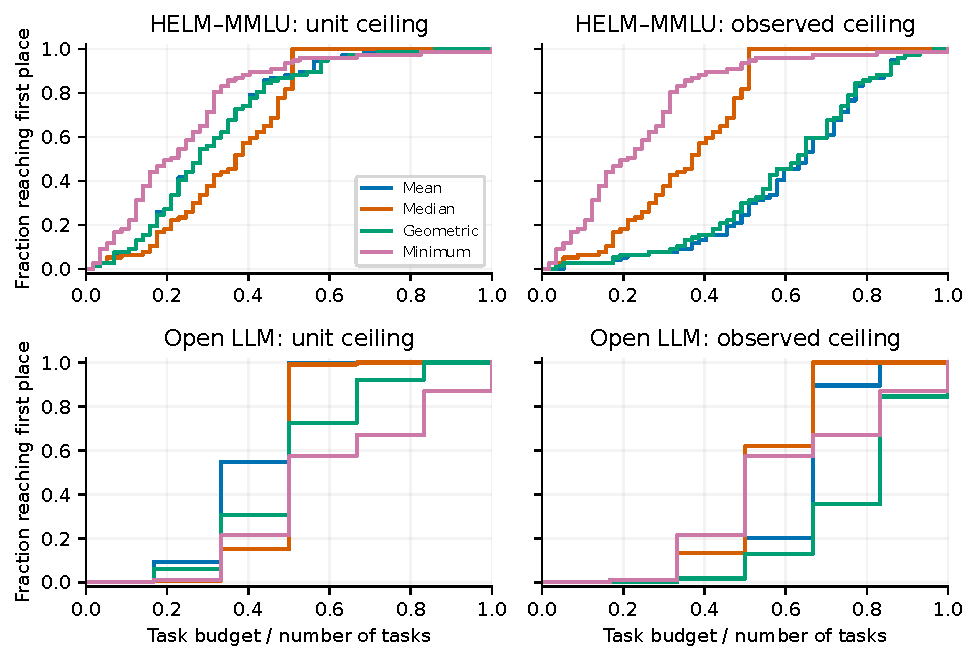
\includegraphics[width=\linewidth]{figures/frontiers.pdf}
\caption{Exact fraction of common challengers that can reach first place within
each task budget at $\rho=1$. Crossings and ceiling dependence prevent a uniform
rule ranking. The steps reflect discrete task counts, especially on six-task
Open LLM. All targets reach co-first by the full budget in these scenarios.}
\label{fig:frontiers}
\end{figure}

HELM makes the mechanism particularly clear. Changing from unit to observed
ceilings increases average mean cost from \HelmUnitMeanK{} to
\HelmObservedMeanK{} tasks, while median remains at \HelmUnitMedianK{}.
Enough coordinates can still cross its threshold, while the caps reduce the
aggregate mass obtainable per changed coordinate. Open LLM's even median also
becomes more expensive, from \OllUnitMedianK{} to \OllObservedMedianK{}, but mean
increases more, from \OllUnitMeanK{} to \OllObservedMeanK{}.

Figure~\ref{fig:frontiers} shows why average budgets do not establish a full
dominance claim. On HELM with unit ceilings, the median can be easier for some
large-budget targets even though it is harder on average. The minimum has the
lowest average task count on HELM, but a larger average than mean on Open LLM
(Table~\ref{tab:support}). Its incumbent is defined by the worst task, so enforcing
that lower winning threshold can be cheap. Penalizing weak performance does not
by itself establish resistance to a change in the winning rank.

Targeted task selection is a consequential baseline control under heterogeneous
caps. Under unit ceilings, lowest-first and optimal costs coincide, as predicted
by Proposition~\ref{prop:endpoint}. Under observed ceilings on HELM, lowest-first
requires \HelmObservedMedianWeakK{} tasks on average for median, versus the optimum
\HelmObservedMedianK{}. The gap arises because spending on the weakest scores can
fail to cross the incumbent's high median boundary. Random ordering is also
substantially more costly (Appendix~\ref{app:baselines}); it cannot establish a
lower bound on an informed developer's investment.

\subsection{Weaker improvements can make winning impossible}
\label{sec:rho}
A small task count under an optimistic ceiling does not imply a reachable training
outcome. Figure~\ref{fig:reachability} gives feasibility even when every task may
be changed. With unit ceilings at $\rho=.5$, the feasible fractions on Open LLM
are \OllUnitHalfMeanFeasible\% for mean and \OllUnitHalfMedianFeasible\% for
median. Under observed ceilings they fall to \OllObservedHalfMeanFeasible\% and
\OllObservedHalfMedianFeasible\%. On HELM, observed-ceiling feasibility at the
same response is \HelmObservedHalfMeanFeasible\% and
\HelmObservedHalfMedianFeasible\%.
These failures are exact consequences of $g(u)<t$, not optimization timeouts.
We report feasibility rather than assign finite effort to such cases. Because
neither ceiling nor $\rho$ is learned from training interventions, the audit
cannot select which of these regimes describes an actual developer.

\begin{figure}[t]
\centering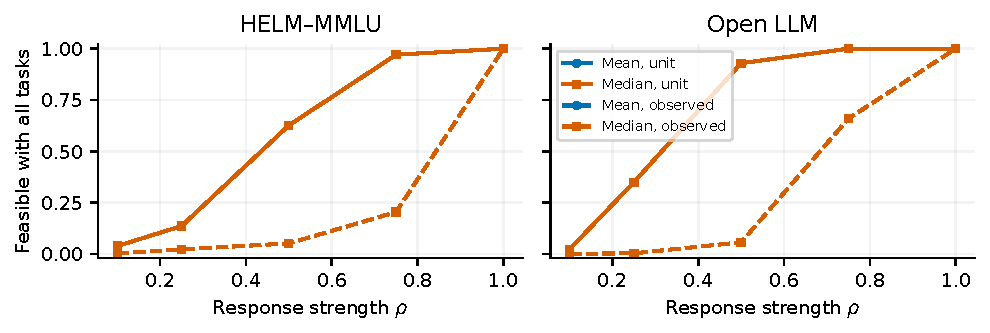
\includegraphics[width=\linewidth]{figures/reachability.pdf}
\caption{Fraction of the fixed common challenger cohort for which winning is
feasible with all tasks available. Solid lines use unit ceilings; dashed lines
use observed ceilings. A larger task budget cannot rescue a target whose full
attainable vector remains below the incumbent.}
\label{fig:reachability}
\end{figure}

\subsection{Counting tasks and counting score increases give different answers}
\label{sec:mass}
Table~\ref{tab:mass} changes the investment unit while keeping scores, rivals,
and thresholds fixed. On unit-ceiling HELM, median needs less score mass than mean
for \HelmUnitMassLess\% of targets, even though it needs more changed coordinates
for \HelmUnitMedMore\%. Its average minimum increase is
\HelmUnitMedianMass{} percentage points per task versus
\HelmUnitMeanMass{} for mean. On Open LLM the corresponding values are
\OllUnitMedianMass{} and \OllUnitMeanMass{}, with median cheaper for
\OllUnitMassLess\% of targets. Thus interpreting task count as total training
effort could reverse an audit's practical message.

\begin{table}[t]
\centering\small\setlength{\tabcolsep}{4pt}
\begin{tabular}{llrrrrr}
\toprule
Panel & Ceiling & Mean & Median & Geom. & Min. & $C_{\rm med}<C_{\rm mean}$ (\%) \\
\midrule
HELM--MMLU & Unit & 14.56 & 3.44 & 14.10 & 3.09 & 100.00 \\
HELM--MMLU & Observed & 14.56 & 3.72 & 14.29 & 3.09 & 100.00 \\
Open LLM & Unit & 30.25 & 18.44 & 25.79 & 8.52 & 99.93 \\
Open LLM & Observed & 30.25 & 18.81 & 26.99 & 8.52 & 99.93 \\
\bottomrule
\end{tabular}

\caption{Mean minimum \emph{average score increase} $100C^*$, in percentage
points, at $\rho=1$. The final column is a paired comparison of score mass.
This is a different optimization from saturating a minimum number of tasks.}
\label{tab:mass}
\end{table}

The mean's mass optimum is exactly its gap to the best rival and is unchanged by
the ceiling whenever feasible. The odd median instead pays just the cheapest
deficits needed to populate its upper half. It can therefore be insensitive to
many very low scores. The minimum ignores no deficit below its own winning
threshold, yet that threshold can be much lower than a mean or median threshold.
The empirical mass distributions are shown in Appendix~\ref{app:massplots}.
Neither investment unit includes task-specific acquisition difficulty or a cost
for changing a model's representation.

\paragraph{An exact overhead--gain tradeoff.}
For the mean and the odd-dimensional median, there is an intervention that
simultaneously attains minimum support and minimum score mass
(Appendix~\ref{app:mixed}). Thus a cost with normalized task overhead
\begin{align}
 J^*_{\lambda,g}&=\min_{x\le y\le u,\ g(y)\ge t}
 \left\{\lambda\frac{\|y-x\|_0}{d}+(1-\lambda)\frac{\|y-x\|_1}{d}\right\}\nonumber\\
 &=\lambda\frac{K^*_g}{d}+(1-\lambda)C^*_g
 \label{eq:mixed}
\end{align}
can be computed exactly from our certificates. This identity is not asserted
for an even median or the geometric mean. On unit-ceiling HELM,
\MixedSwitchers{} challengers switch from median cheaper at $\lambda=0$ to
median costlier at $\lambda=1$. Their crossover weights have median
\MixedMedian{} and interquartile range $[\MixedQOne,\MixedQThree]$.
Under observed ceilings median is never more expensive for any weight in this
cohort (Figure~\ref{fig:mixed}). The weights are hypothetical cost ratios,
not fitted training parameters. They expose which notion of investment is
responsible for a robustness claim.

\begin{figure}[t]
\centering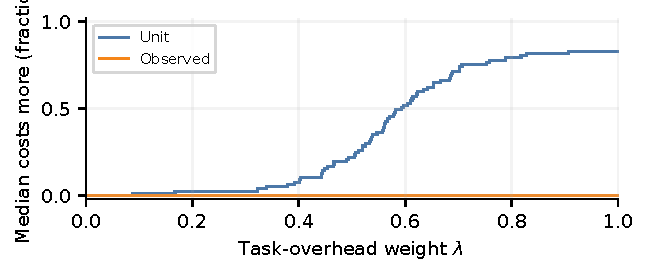
\includegraphics[width=.73\linewidth]{figures/mixed_cost.pdf}
\caption{Exact mixed-cost comparison on HELM at $\rho=1$. The vertical axis
is the fraction of common challengers with $J^*_{\lambda,\med}>
J^*_{\lambda,\mean}$. A larger overhead weight can reverse the unit-ceiling
comparison, while observed-ceiling median costs never exceed mean costs here.}
\label{fig:mixed}
\end{figure}

\subsection{Sensitivity and what uncertainty means here}
\label{sec:uncertainty}
These tables are censuses of two retained snapshots, so their optimization results
have no Monte Carlo estimation error. The central uncertainties concern what
counts as a task, which models are represented, and what gains training can attain.
We expose the first two through two reproducible perturbations. We resample owner
groups of targets, using the model namespace as a coarse cluster, and compute
2,000 paired reweightings. Separately, we draw 300 task multisets with replacement,
preserve their original dimension, recompute all competing thresholds and caps,
and retain the original target cohort. Table~\ref{tab:uncertainty} reports their
central 95\% ranges for the mean paired difference $\Delta K=K^*_\med-K^*_\mean$.
These are sensitivity ranges, not confidence intervals for independent models,
unseen tasks, or true test accuracy.

\begin{table}[t]
\centering\small\setlength{\tabcolsep}{4pt}
\begin{tabular}{llrrr}
\toprule
Panel & Ceiling & $100\overline{\Delta K/d}$ & Owner reweighting & Task resampling \\
\midrule
HELM--MMLU & Unit & 4.74 & [2.19, 6.96] & [-0.07, 11.14] \\
HELM--MMLU & Observed & -26.57 & [-28.61, -24.71] & [-34.03, -21.17] \\
Open LLM & Unit & 8.12 & [6.93, 9.26] & [-2.30, 15.72] \\
Open LLM & Observed & -10.70 & [-11.42, -9.99] & [-32.46, 2.71] \\
\bottomrule
\end{tabular}

\caption{Paired task-count difference as a percentage of panel dimension.
Positive means median costs more. Owner reweighting and task resampling are
different perturbations of a finite table, not statistical evidence about a
random population.}
\label{tab:uncertainty}
\end{table}

Owner reweighting preserves the signs of all four average differences in these
ranges. Task perturbation is less stable: both unit-ceiling intervals cross zero,
as does the observed-ceiling Open LLM interval. The observed-ceiling HELM contrast
is more stable within this particular perturbation. Repeated heterogeneous tasks
should be interpreted as a change of benchmark emphasis, not a plausible sample
of newly collected evaluation questions.

The main direction of the ceiling reversal persists among the top 20\% by original
mean rank and when retaining all unflagged evaluation entries. Moving Open LLM
from displayed normalized columns to raw metric columns reduces the observed-ceiling
fraction with median cheaper from \OllObservedMedLess\% to \OllRawObservedMedLess\%: most cases
then tie in task count. This is a substantive scale limitation, not evidence for
normalization invariance. A positive winning margin changes some HELM budgets
but preserves the reversal; no Open LLM budget changes in this check.
Evaluation-instance weighting also changes HELM mean budgets. Full controls and
per-rule incumbents appear in Appendix~\ref{app:controls}.

\section{Discussion and limitations}
\label{sec:discussion}
The answer to ``how much investment is needed?'' is a conditional frontier, not
one number. A leaderboard designer can publish $(K^*,C^*)$ against explicit
attainability scenarios, show where winning is impossible, and inspect witnesses
near incumbent boundaries. The designer must still choose a scientific objective.
A rule that makes rank change difficult may merely encode a different notion of
quality or a low bottleneck threshold. Our results do not recommend minimum,
mean, or median as an overall evaluation policy.

The principal limitation is identification. Public scores contain no intervention
data mapping domain-specific training examples to gains, spillovers, or forgetting.
Observed task maxima are attainable by some entry individually, not necessarily
jointly or by the target. Saturation can overstate what post-training achieves;
no negative transfer can understate its cost. Unequal task sizes and metrics make
uniform task count and uniform score mass incomplete proxies. Even continuous
score changes idealize the discrete increments of finite accuracy tests. Our
formulas concern reported scores, and we cannot attach test-item confidence
intervals without corresponding example-level outputs and a defensible sampling model.

The data are historical, selected, and contain correlated model families. Owner
clusters imperfectly capture shared lineage; the small number of heterogeneous
Open LLM task groups limits any task-general claim. A task-group attack may mean
improving many subtasks, whereas a HELM coordinate is one subject. Ordinal
aggregators, hidden evaluations, and responding rivals require other optimization
models. The literature protocol was intentionally restricted; no exhaustive
related-work or novelty certification is claimed. None of the computed witnesses
establishes contamination by any named model, and no model was trained here.

\section{Conclusion}
Exact score-space certificates make the required assumptions visible. On two public
leaderboards, changing only the improvement ceiling reverses the average task-count
comparison of mean and median; changing the investment unit changes it again.
The same analysis also identifies unreachable winners and sensitivity to benchmark
composition. Claims about aggregation and strategic investment should therefore
specify the attainable gains, winning convention, task unit, and cost measure.
\label{endmain}

\clearpage
\section*{AI use statement}
This report was produced by an autonomous Codex research agent in response to a
user-specified task. AI was used for conceptual modeling, mathematical statements
and proofs, hypothesis formulation, experimental design, implementation, data
cleaning, quantitative analysis, interpretation, literature selection and reading,
figures, and all manuscript drafting and editing. No benchmark examples or
empirical scores were generated by an AI model. The numerical results come from
executed code on downloaded public score tables. Automated validation includes
exhaustive searches, independently formulated optimization checks, and endpoint
witness audits. This is not independent human review, and no human verification
of the paper is claimed. No models were trained, and no paid inference API was
used for experiments. The report is a research deliverable, not a submission to
or publication at ICLR.

\section*{Ethics statement}
The study uses public aggregate evaluation scores without private user data or
human-subject experiments. No benchmark was contaminated and no evaluated model
was modified. Minimum-investment witnesses describe potential score sensitivity;
they are not allegations against developers. Such audits can help benchmark
maintainers identify fragile incentive structures, while also revealing how a
known aggregation rule could be targeted. We release score-space analysis rather
than training or data-leakage pipelines. Data-source cards do not declare a separate
score-data license; the artifact records this uncertainty and makes no claim that
the underlying models' licenses license leaderboard data.

\section*{Reproducibility statement}
The artifact contains the LaTeX source, the official unmodified ICLR 2027 style,
pinned dependencies, frozen score summaries, SHA-256 checksums and source URLs,
complete processing and experiment scripts, model-level results, and generated
tables and plots. Equations~\ref{eq:k}--\ref{eq:median} and
Appendix~\ref{app:proofs} specify the algorithms. Appendix~\ref{app:repro} and
\texttt{README.md} give exact commands, seeds, runtime, and the table/figure map.
The access protocol in \texttt{RESEARCH\_LOG.md} records the restricted literature
review, failed URL probes, and development runs. A completed artifact checklist
appears in Appendix~\ref{app:checklist}; the inspected ICLR instructions require
the AI statement above, rather than a NeurIPS-style paper checklist.

\bibliography{references}
\bibliographystyle{iclr2027_conference}

\clearpage
\appendix
\section{Proofs and exact algorithms}
\label{app:proofs}
\subsection{Endpoint reduction and shared ceilings}
\begin{proof}[Proof of Proposition~\ref{prop:endpoint}]
For a feasible $y$, let $S=\{j:y_j>x_j\}$. Set $z_j=u_j$ for $j\in S$ and
$z_j=x_j$ otherwise. Then $z\ge y$ coordinatewise, hence $g(z)\ge g(y)$, and its
support has size at most $|S|$. This proves endpoint sufficiency without convexity
or symmetry. If all endpoints equal $c$, consider a selected coordinate with
original value $b$ and an unselected coordinate with original value $a\le b$.
The resulting pair is $(a,c)$. Exchanging selection gives $(b,c)$, whose sorted
coordinates are no smaller. After inserting the other unchanged coordinates,
the entire sorted vector is also coordinatewise no smaller. Symmetry allows us
to compare these sorted vectors, and monotonicity prevents a decrease in $g$.
Repeating exchanges selects the $k$ smallest original values. An intervention on
fewer than $k$ coordinates can be extended without decreasing its value. Thus
the result holds for ``at most $k$'' as well.
\end{proof}

This result does not cover unequal task weights, heterogeneous caps, or a common
fractional response $\rho<1$. In the last case the endpoints increase with the
original scores, and an exchange changes both sorted endpoints. For the mean and
geometric mean under a unit ceiling, sorting gains nevertheless remains exact
at every response strength.

\subsection{Support formulas, zeros, and infeasibility}
\begin{proof}[Proof of Proposition~\ref{prop:support}]
For mean aggregation, saturation on subset $S$ increases the unnormalized sum by
$\sum_{j\in S}(u_j-x_j)$. Among size-$k$ subsets this is maximized by the largest
$k$ gains, proving Equation~\ref{eq:mean}. The empty prefix is allowed, and no
prefix large enough means infeasibility. For the geometric mean with positive
coordinates, use $\sum_j\log y_j\ge d\log t$ and gains
$\log u_j-\log x_j$. If $t>0$, every zero original coordinate must be selected
and must have $u_j>0$. Replace these zeros by their caps to form a base log sum,
then sort the log gains of the remaining positive coordinates. Add the mandatory
zero count to the required prefix length. If any zero has zero cap, winning is
impossible. For $t\le0$, a nonnegative score vector is already feasible.

For $d=2m-1$, its median is at least $t$ precisely when at least $m$ coordinates
are at least $t$. Exactly $A$ already satisfy this, and at most $B$ can ever
satisfy it. Any $m-A$ eligible coordinates below $t$ suffice when $B\ge m$.
The minimum is at least $t$ if and only if every coordinate is at least $t$,
which gives its formula. Finally, monotonicity implies that $g(u)$ is the maximum
attainable score; hence $g(u)\ge t$ is necessary and sufficient for feasibility.
\end{proof}

At $\rho=1$, $\eps=0$, and $u_j=\max_\ell X_{\ell j}$, the best rival's vector
is coordinatewise bounded by $u$. An odd-median rival at score $t$ has at least
$m$ coordinates at or above $t$, ensuring $B\ge m$; its support cost is then
$(m-A)_+$ under both observed and unit ceilings. For the minimum, all observed
caps are at least the best rival's minimum, so the same original deficits must
be changed under either ceiling. This establishes the co-first invariances
stated in Section~\ref{sec:methods}. It does not assert equality of continuous
median costs, nor feasibility with a positive margin above that rival.

The even median is not replaced by either central order statistic. The code
enumerates all 64 subsets when $d=6$, sorts their improved score vectors, averages
the central pair, and returns the minimum feasible subset cardinality. This is an
exact exponential algorithm restricted to a small dimension, not a claimed
polynomial algorithm for arbitrary even $d$. Weighted means are also exact:
sort gains $w_j(u_j-x_j)$ and cover $t-\sum_jw_jx_j$, where $\sum_jw_j=1$.

\subsection{No uniform ordering and a ceiling reversal}
\begin{proof}[Proof of Proposition~\ref{prop:flip}]
Use the construction in the main text. Each specialist has mean $.604/3<.60$
and median zero, so the uniform incumbent sets both thresholds. With unit caps,
one changed target coordinate raises its mean to $(1+.59+.59)/3>.60$, while its
median remains $.59$. Two changes suffice for the median. With observed caps
$.604$ on each coordinate, two changes give a mean
$(.604+.604+.59)/3<.60$; three give $.604$. Two changes give median $.604$.
These strict comparisons persist at a $10^{-6}$ margin, as also checked in code.
Only the cap model has changed. The target, rivals, rules and task units are fixed.
\end{proof}

The reverse task-count ordering can already occur at a unit ceiling: against
incumbent $(.6,.6,.6)$, a target $(0,.1,.61)$ needs two changed tasks for mean but
only one for median. A single mean improvement yields at most $(1+.1+.61)/3=.57$,
whereas changing the $.1$ coordinate makes the median $.61$. These examples rule
out deterministic dominance over all score tables. They are mathematical proof
constructions, explicitly excluded from every empirical table and figure.

\subsection{Continuous score-mass investment}
\label{app:mass}
Assume the target is below threshold and that the endpoint vector is feasible.
For the mean, the required total gain is $dt-\sum_jx_j$. A box allows every total
gain between zero and $\sum_j(u_j-x_j)$, so this gain is both necessary and
attainable. Dividing by $d$ gives the mean formula. For the minimum, every
deficit $(t-x_j)_+$ must be paid; summing these independent necessities is
attainable whenever all caps cross the threshold.

For the odd median, assign cost $b_j=(t-x_j)_+$ to any coordinate with $u_j\ge t$
and $b_j=+\infty$ otherwise. At least $m$ coordinates must reach $t$, and each
has exactly that minimum cost. Therefore
\begin{equation}
 C^*_\med=d^{-1}\sum_{r=1}^{m}b_{[r]},
\end{equation}
where $b_{[r]}$ are sorted increasingly. Zero costs account for coordinates
already above threshold. Infeasibility is retained if fewer than $m$ finite
costs exist.

For the geometric mean at $t>0$, minimize $\sum_j(y_j-x_j)$ subject to the box
and $\sum_j\log y_j\ge d\log t$. This is a convex feasible region. The
Lagrangian stationarity condition on an interior coordinate is
$1-\lambda/y_j=0$. Hence
\begin{equation}
 y_j=\min\{u_j,\max\{x_j,\lambda\}\},\qquad
 \sum_j\log y_j=d\log t.
\end{equation}
Monotonicity gives a one-dimensional root; the code uses Brent's method with
absolute root tolerance $10^{-14}$. Clamped flat segments do not change the
minimum attained mass. An infeasible endpoint or a zero cap at a positive
threshold is handled before root finding.

For an even dimension $d=2m$ (six in our data), median feasibility means that
$y_{(m)}\ge a$ and $y_{(m+1)}\ge b$ for some $a\le b$ with $a+b=2t$.
Choose a set $H$ of $m$ coordinates to reach $b$ and one additional coordinate
$\ell\notin H$ to reach $a$. The others stay unchanged. For this assignment,
the total cost as a function of $a$ is
\begin{equation}
 f_{H,\ell}(a)=\sum_{j\in H}(2t-a-x_j)_+ +(a-x_\ell)_+,
\end{equation}
on the interval
\begin{equation}
 \max\{0,2t-\min_{j\in H}u_j\}\le a\le\min\{t,u_\ell\}.
\end{equation}
Empty intervals are infeasible. Otherwise this piecewise-linear convex function
attains a minimum at an endpoint or a breakpoint $a=x_\ell$ or $a=2t-x_j$.
We evaluate those clipped candidates and minimize over all $(H,\ell)$.
For necessity, take the top $m$ coordinates and the next coordinate of any
feasible $y$, set $a=y_{(m)}$ and $b=2t-a\le y_{(m+1)}$, and reduce unnecessary
increases. If $y_{(m)}>t$, one may instead set $a=b=t$. Thus the enumeration
covers an optimum. No relaxation is used.

\subsection{Joint attainment for mixed overhead and score cost}
\label{app:mixed}
For a feasible mean threshold above the original score, choose a minimum-support
set of largest headrooms. Its total headroom covers $dt-\sum_jx_j$, whereas
every smaller set fails to cover that gap. Allocate exactly that total gain over
the chosen coordinates. Such an allocation exists in the box; if any chosen
coordinate had zero gain, a smaller support would cover the gap, a contradiction.
This intervention attains both $K^*_\mean$ and $C^*_\mean$.
For an odd median, write $K=m-A>0$. Choose the $K$ smallest positive deficits
among coordinates whose caps reach $t$, and raise them exactly to $t$.
Together with the $A$ already qualifying coordinates, this attains both the
minimum support and the minimum mass. If the target already wins, the zero
intervention attains both. Any nonnegative weighted sum of two separately
minimized costs is at least the corresponding weighted sum of their minima;
these common optimizers attain equality, proving Equation~\ref{eq:mixed}.
This proof requires neither shared caps nor full saturation, but does require
feasibility. The figure uses the feasible $\rho=1$ HELM cohort.
When $\Delta s=(K^*_\med-K^*_\mean)/d>0$ and
$\Delta c=C^*_\med-C^*_\mean<0$, the crossover is exactly
$\lambda_*=-\Delta c/(\Delta s-\Delta c)$.

\section{Data and experimental controls}
\label{app:controls}
\subsection{Acquisition, completeness, and score units}
The download script requests the frozen HELM release listing, its release summary,
and exactly the 57 files matching
\texttt{groups/json/mmlu\_mmlu\_subject:*.json}; similarly named alternative
group tables are not duplicated. Each subject table has one run specification per
row, from which the model identifier is parsed. We extract its \texttt{EM} column
and retain evaluation counts for the micro-mean control. All 79 identifiers occur
in every subject. The Open LLM parquet and dataset card are downloaded at the full
commit in \texttt{data/manifest.json}. In total the manifest covers \RawFiles{}
raw files, \RawMB{} MB. No full run-output collection or evaluation-set examples
are needed.

The Open LLM precision priority is bfloat16, float16, float32, 8bit, 4bit, then
other labels. Ties use lexicographic \texttt{eval\_name}; the first row per
\texttt{fullname} is kept. This rule consults no scores. The full-entry sensitivity
keeps all complete, unflagged \texttt{eval\_name} records. The raw-score
sensitivity uses the same selected rows and the six \texttt{Raw} columns without
dividing them by 100, since those columns are already on the unit scale.
These two scales have different task-specific baselines and are not related by
a common monotone transformation of the aggregate. Macro scores are carried to
CSV with 17 significant digits.

\begin{table}[h]
\centering\small\setlength{\tabcolsep}{3pt}
\begin{tabular}{llrp{6.1cm}}
\toprule
Panel & Rule & Maximum & Entry / model \\
\midrule
HELM--MMLU & Mean & 0.872730 & anthropic\_claude-3-5-sonnet-20241022 \\
HELM--MMLU & Median & 0.898148 & anthropic\_claude-3-5-sonnet-20241022, deepseek-ai\_deepseek-v3 \\
HELM--MMLU & Geometric & 0.867504 & deepseek-ai\_deepseek-v3 \\
HELM--MMLU & Minimum & 0.596386 & deepseek-ai\_deepseek-v3 \\
Open LLM & Mean & 0.520814 & MaziyarPanahi/calme-3.2-instruct-78b \\
Open LLM & Median & 0.556164 & ehristoforu/qwen2.5-test-32b-it \\
Open LLM & Geometric & 0.472896 & MaziyarPanahi/calme-3.2-instruct-78b \\
Open LLM & Minimum & 0.231464 & rootxhacker/Apollo-70B \\
\bottomrule
\end{tabular}

\caption{Initial competing thresholds and winners under each audited rule.
HELM median has a tie. These entries remain in every target's rival set.}
\label{tab:leaders}
\end{table}

The original Open LLM score table contains model hub-license metadata but no
dataset-level license declaration. Neither the inspected HELM summaries nor the
public release listing states a separate score-data license. Access without an
account does not establish an open-data license, and HELM code's Apache license
is not assumed to apply to these scores. This artifact uses aggregate scores for
reproducibility and records sources and checksums, without asserting third-party
redistribution rights. A fresh-download path is provided.

\subsection{Alternative target cohorts and normalization}
\begin{table}[h]
\centering\small\setlength{\tabcolsep}{3pt}
\begin{tabular}{llrrrr}
\toprule
Panel / cohort & Ceiling & Targets & Mean $K$ & Median $K$ & Median cheaper (\%) \\
\midrule
HELM--MMLU top 20\% & Unit & 14 & 5.71 & 7.71 & 14.3 \\
HELM--MMLU top 20\% & Observed & 14 & 17.43 & 7.71 & 85.7 \\
Open LLM top 20\% & Unit & 897 & 1.54 & 2.26 & 0.0 \\
Open LLM top 20\% & Observed & 897 & 3.03 & 2.29 & 71.3 \\
Open LLM (raw) & Unit & 4494 & 2.35 & 2.93 & 0.0 \\
Open LLM (raw) & Observed & 4494 & 3.66 & 3.61 & 11.0 \\
Open LLM (all entries) & Unit & 4572 & 2.36 & 2.85 & 0.0 \\
Open LLM (all entries) & Observed & 4572 & 3.88 & 3.24 & 62.4 \\
\bottomrule
\end{tabular}

\caption{Exact $\rho=1$ task-count controls. ``Top 20\%'' means mean rank at
most $\lceil .2n\rceil$, then common nonleader exclusion. Raw and full-entry
panels each recompute incumbents and their own common cohort.}
\label{tab:cohorts}
\end{table}
The top-cohort control preserves the direction of the primary mean--median
comparison for both ceilings. The raw-column observed-ceiling comparison is much
closer to a tie; results on one normalization should not be generalized to another.
Full-entry retention changes the fractions only slightly in this snapshot but
does not eliminate the more general problem of dependent model submissions.

\subsection{Winning margins and subject weighting}
\begin{table}[h]
\centering\small\setlength{\tabcolsep}{3pt}
\begin{tabular}{llrrrr}
\toprule
Panel & Ceiling & Any $K$ changed & Mean $K$ & Median $K$ & Median cheaper (\%) \\
\midrule
HELM--MMLU & Unit & 7 & 17.12 & 19.90 & 14.3 \\
HELM--MMLU & Observed & 7 & 34.96 & 19.90 & 97.4 \\
Open LLM & Unit & 0 & 2.36 & 2.85 & 0.0 \\
Open LLM & Observed & 0 & 3.88 & 3.24 & 62.5 \\
\bottomrule
\end{tabular}

\caption{Positive-margin control ($\eps=10^{-6}$), $\rho=1$.
``Any $K$ changed'' counts targets whose support budget changes for at least
one of the four rules relative to co-first. All remain feasible.}
\label{tab:ties}
\end{table}

\begin{table}[h]
\centering\small
\begin{tabular}{lrrrr}
\toprule
Ceiling & Targets & Macro mean $K$ & Micro mean $K$ & Different $K$ (\%) \\
\midrule
Unit & 78 & 16.91 & 11.27 & 96.2 \\
Observed & 78 & 34.53 & 33.74 & 75.6 \\
\bottomrule
\end{tabular}

\caption{HELM arithmetic mean with equal subject weights (macro) versus weights
proportional to evaluated question counts (micro). Cohort: entries not initially
co-first under either mean, rather than the four-rule cohort of the main audit.}
\label{tab:weighting}
\end{table}
The denominator for this weighting control differs from the main cohort because
only the two mean variants are compared. Task counts still assign unit overhead
to each subject, even when score contributions are weighted by subject size.

\section{Strategy baselines}
\label{app:baselines}
\begin{table}[h]
\centering\small
\begin{tabular}{lllrrr}
\toprule
Panel & Ceiling & Rule & Optimal & Lowest first & Random order \\
\midrule
HELM--MMLU & Unit & Mean & 17.12 & 17.12 & $27.94\pm0.01$ \\
HELM--MMLU & Unit & Median & 19.82 & 19.82 & $22.48\pm0.01$ \\
HELM--MMLU & Unit & Geometric & 17.35 & 17.35 & $30.71\pm0.02$ \\
HELM--MMLU & Unit & Minimum & 13.52 & 13.52 & $51.43\pm0.04$ \\
HELM--MMLU & Observed & Mean & 34.96 & 36.53 & $46.69\pm0.02$ \\
HELM--MMLU & Observed & Median & 19.82 & 43.31 & $44.15\pm0.03$ \\
HELM--MMLU & Observed & Geometric & 34.13 & 35.26 & $47.41\pm0.02$ \\
HELM--MMLU & Observed & Minimum & 13.52 & 13.52 & $51.35\pm0.04$ \\
Open LLM & Unit & Mean & 2.36 & 2.36 & 2.74 \\
Open LLM & Unit & Median & 2.85 & 2.85 & 3.02 \\
Open LLM & Unit & Geometric & 2.98 & 2.98 & 3.95 \\
Open LLM & Unit & Minimum & 3.66 & 3.66 & 5.36 \\
Open LLM & Observed & Mean & 3.88 & 4.84 & 4.82 \\
Open LLM & Observed & Median & 3.24 & 5.23 & 5.18 \\
Open LLM & Observed & Geometric & 4.65 & 4.70 & 5.31 \\
Open LLM & Observed & Minimum & 3.66 & 3.66 & 5.36 \\
\bottomrule
\end{tabular}

\caption{Mean number of tasks before reaching co-first, $\rho=1$.
Lowest-first orders by original task scores. Random-order expectation is exact
over subsets on Open LLM and estimated using 256 independent random permutations
per target on HELM (seed 20261102); $\pm$ gives one Monte Carlo standard error
of the finite-cohort mean, propagating independent target-wise draw variances.
The optimal and lowest-first entries coincide
at unit ceilings as a theorem, not a numerical coincidence.}
\label{tab:baselines}
\end{table}
For a random permutation and budget $k$, its first $k$ tasks are uniformly
distributed over size-$k$ subsets. If $p_k$ is the fraction of such subsets that
win, monotonicity yields $\mathbb{E}K=\sum_{k=0}^{d-1}(1-p_k)$ whenever the full
budget is feasible. We enumerate those fractions on the six-task panel. For
HELM, permutation draws estimate this expectation; they are a randomized
baseline, not part of the exact optimum. The artifact also records $\rho=.5$
baseline outcomes, but does not average their infeasible codes as finite effort.
The full model-level outputs allow different budget thresholds to be inspected.

\section{Additional distributions}
\label{app:massplots}
\begin{figure}[h]
\centering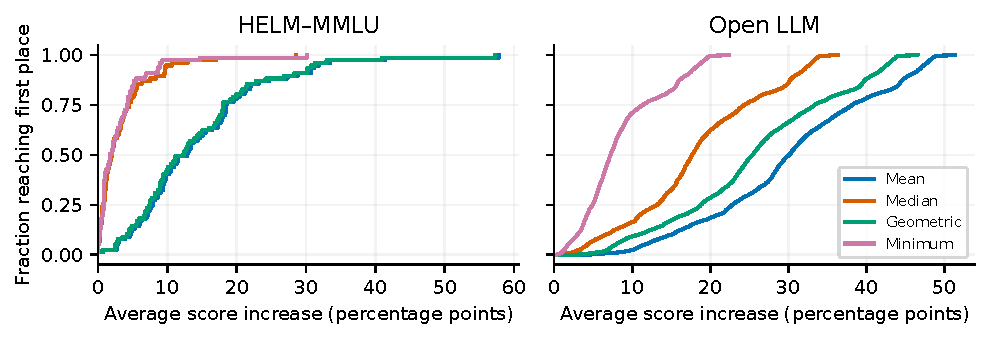
\includegraphics[width=\linewidth]{figures/mass.pdf}
\caption{Exact continuous score-mass frontiers under unit ceilings at $\rho=1$.
The horizontal unit is average percentage-point increase across a panel's tasks,
not training examples or compute. These curves solve Equation~\ref{eq:c}.}
\label{fig:mass}
\end{figure}

\begin{figure}[h]
\centering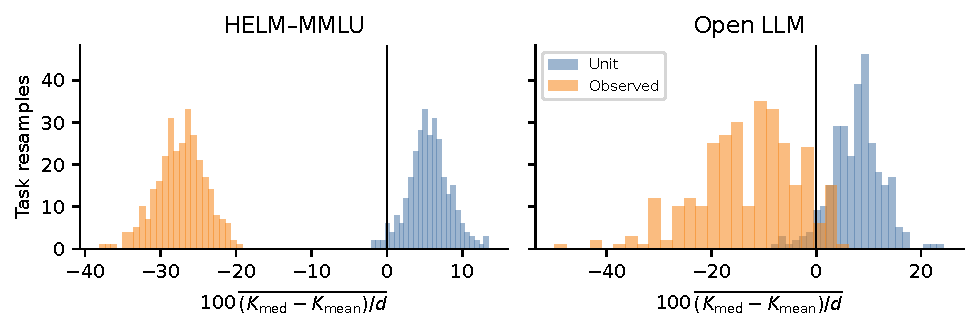
\includegraphics[width=\linewidth]{figures/task_perturbations.pdf}
\caption{Mean paired support difference over 300 task multisets per panel.
Within a draw, all models share the same sampled tasks and thresholds and caps
are recomputed. The original common target cohort is held fixed. Crossing zero
indicates that changing task emphasis can change the comparison.}
\label{fig:tasks}
\end{figure}
The bootstrap is used only as a controlled perturbation of benchmark composition.
It does not repair missing training-response information. In particular, replicating
one of six heterogeneous Open LLM groups can substantially change the scientific
meaning of the benchmark. This is precisely why the broad observed-ceiling
comparison on that panel is weaker than a universal robustness claim.

\section{Reproduction details}
\label{app:repro}
The environment is Python 3.11.2, NumPy 2.2.6, pandas 2.3.3, SciPy 1.15.3,
Matplotlib 3.10.7, PyArrow 22.0.0, and requests 2.32.5. Full transitive versions
are in \texttt{requirements-lock.txt}; TeX uses the official ICLR 2027 style
downloaded from the URL in its author guidelines. The style files are unchanged.
Only the running header is set in the manuscript to avoid suggesting publication
or an actual conference submission. We enforce the initial-submission nine-page
main-text ceiling. AI, ethics, and reproducibility statements, references, and
appendices are outside that limit according to the inspected instructions.

From the artifact root, create a virtual environment, install the pinned
requirements, and run the following commands:
\begin{verbatim}
python -m src.fetch_data
python -m src.prepare_data
OPENBLAS_NUM_THREADS=1 OMP_NUM_THREADS=1 \
  python -m src.run_experiments --task-bootstrap 300
OPENBLAS_NUM_THREADS=1 python -m src.report
python -m pytest -q
cd paper && latexmk -pdf -interaction=nonstopmode main.tex
\end{verbatim}
The download step verifies existing frozen files against the manifest instead of
silently replacing them. Internet access is only needed for a fresh download.
Processing, experiments, plots and PDF compilation can be rerun offline with the
included raw scores. The recorded main run takes \RunWallSeconds{} seconds wall
time and \RunCpuSeconds{} process CPU seconds with BLAS/OpenMP limited to one
thread; actual speed varies by host. It uses \RunPeakMiB{} MiB peak resident
memory. No GPU, model execution, or paid API is needed.

The master seed is 20261102 for random-order baselines, 20261103 for task
multisets, and 20261104 for owner-group reweighting. Exact optimization itself has
no random seed. Coarse HELM owners use the identifier prefix before the first
underscore; Open LLM owners use the namespace before the slash. In owner
reweighting, entire groups are sampled with replacement, and both numerator and
denominator of the paired target mean are reweighted together. This retains
within-group dependence as represented by that imperfect proxy.

Every paper table and figure is generated by \texttt{src/report.py} from
\texttt{artifacts/*.csv}. Source scores and optimization results come from
\texttt{prepare\_data.py} and \texttt{run\_experiments.py}. Specifically,
Table~\ref{tab:support} uses \texttt{support.csv}; Table~\ref{tab:mass} and
Figure~\ref{fig:mass} use \texttt{mass.csv}; Table~\ref{tab:uncertainty} and
Figure~\ref{fig:tasks} additionally use \texttt{task\_bootstrap.csv} and namespace
metadata. Figures~\ref{fig:frontiers} and~\ref{fig:reachability} and
Tables~\ref{tab:cohorts} and~\ref{tab:ties} use \texttt{support.csv}.
Table~\ref{tab:leaders} aggregates processed matrices directly;
Table~\ref{tab:weighting} uses \texttt{weighting.csv};
Table~\ref{tab:baselines} uses \texttt{baselines.csv} and \texttt{support.csv}.
Figure~\ref{fig:mixed} uses the mean and odd-median columns of
\texttt{support.csv} and \texttt{mass.csv}, writing the exact derived curves to
\texttt{mixed\_cost.csv} and target crossover weights to
\texttt{mixed\_crossovers.csv}.
\texttt{generated/numbers.tex} supplies narrative empirical numbers.

In storage only, infeasible $K^*$ is encoded as $d+1$, never as a measured finite
investment; infeasible mass is infinity. All reported mean support costs use
$\rho=1$, where the cohorts are feasible. Partial-response figures use feasibility
indicators. \texttt{witnesses.json} contains selected target/task lists and
before/after scores. \texttt{witness\_audit.json} records the full audit count.
The tests compare all four support solvers against exhaustive search with zeros,
ties, and nonuniform caps; independent LP and constrained-optimization checks
cover continuous median and geometric costs. Proof constructions are tested as
well, but never included as empirical data.

\section{Completed reporting and artifact checklist}
\label{app:checklist}
The inspected ICLR 2027 author guidelines and official template require an AI use
statement and recommend ethics and reproducibility statements. Those are completed
above. They do not prescribe a separate NeurIPS-style paper checklist. The following
additional checklist documents this deliverable's claims and limits.
\begin{enumerate}
\item \textbf{Claims bounded by evidence: Yes.} Every empirical statement concerns
the frozen panels and declared gain boxes. No training-cost or misconduct inference
is made (Sections~\ref{sec:setup} and~\ref{sec:discussion}).
\item \textbf{Assumptions and proof coverage: Yes.} Bounds, no spillovers, fixed
rivals, ties, zeros, feasibility and even-median handling are explicit. Full proofs
appear in Appendix~\ref{app:proofs}.
\item \textbf{Data provenance and selection: Yes.} Versions, URLs, checksums,
precision priority, dropped records and licensing uncertainty are recorded in
the artifact and Appendix~\ref{app:controls}.
\item \textbf{Reproducible code and environment: Yes.} Pinned requirements, seeds,
commands, exact score matrices, per-target results and scripts for every table
and figure are included (Appendix~\ref{app:repro}).
\item \textbf{Baselines and ablations: Yes.} Lowest-first, random order,
partial responses, ceilings, score mass, alternative cohorts and normalization,
positive margins and subject weights are reported.
\item \textbf{Uncertainty: Yes, within scope.} Paired owner reweighting and task
perturbations are reported as sensitivity ranges. Test-item accuracy uncertainty
and uncertainty in training responses are not estimated; the missing information
is stated explicitly.
\item \textbf{Computational resources: Yes.} CPU time and peak memory are logged.
No GPU training, model evaluation or paid experimental API was used.
\item \textbf{Negative and unanticipated results: Yes.} Infeasibility, task-scale
dependence, task-resampling sign changes and the score-mass reversal are retained.
\item \textbf{Human subjects or private data: Not applicable.} Only public aggregate
scores are analyzed. No privacy-sensitive examples are collected.
\item \textbf{AI assistance and human review: Disclosed.} All research and writing
were agent-produced; no independent human review is claimed.
\item \textbf{Restricted access protocol: Followed.} Only the allowed starting
papers, a directly addressed older election-bribery paper, and official data,
software metadata and template/policy pages were consulted. No forward/backward
citation search or attempt to identify the excluded paper was performed. The
access log reports no recognized incidental encounter with excluded material.
\item \textbf{Submission status and format: Complete report, not submitted.}
Official ICLR 2027 files and the nine-page initial main-text limit are used;
there is no claim of peer review or acceptance.
\end{enumerate}
\end{document}
